\chapter{Analisi stabilometriche}
\label{cap:analisi_stabilometriche}

\section{Sull'analisi posturografica}
In questo capitolo tratteremo i concetti base dell'analisi posturografica ponendo particolare attenzione al modello biomeccanico del singolo pendolo inverso utilizzato per estrarre informazioni utili dal movimento e a come, tradizionalmente, tale analisi viene svolta.

L'analisi posturografica (o stabilometrica) permette di valutare la stabilità del paziente in posizione eretta studiando la posizione e la dinamica del baricentro, o per meglio dire, della proiezione del baricentro su un piano parallelo al terreno. L'analisi stabilometrica non misura l'equilibrio in senso letterale, ma la capacità del paziente nel mantenere una posizione eretta equilibrata.

I metodi utilizzati per l'analisi posturografica solitamente possono essere raggruppati in due categorie: {\bfseries\itshape statici} oppure {\bfseries\itshape dinamici}. Nei test statici il paziente è posto in piedi su una superficie di misurazione piana orizzontale (spesso una pedana stabilometrica) con gli occhi aperti oppure chiusi, senza la presenza di alcuna perturbazione esterna; in questo modo si è in grado di stabilire la postura a riposo del paziente. Nei test dinamici la postura è perturbata da stimoli esterni imprevedibili dal paziente in modo da valutare la sua capacità di riprendere la postura iniziale.

Queste tecniche studiano differenti aspetti del sistema di controllo della postura umana e ci permettono di ottenere delle informazioni indipendenti le une dalle altre. La principale differenza è che nel paradigma statico la maggior parte del sistema sensoriale umano è attiva sotto ad una soglia limite (lo si può considerare quindi a riposo) \cite{fitzpatrick93}\cite{konradson96} fatta eccezione dei recettori cutanei plantari \cite{kavounoudias98}\cite{wu97}, mentre nel paradigma dinamico tutti i recettori sono attivi sopra la soglia limite. Un'altra differenza fra questi due sistemi è che nel caso statico l'unica fonte di instabilità nella postura è interna quindi il corpo è in grado di anticipare e correggere i disturbi, mentre nel caso dinamico il disturbo è esterno e non prevedibile.

\section{La pedana di forza}
Per svolgere l'esame stabilometrico esistono vari strumenti, il più popolare è la {\bfseries pedana di forza}.

Il corpo si muove grazie alla combinazione di forze interne, determinate dall'azione dei muscoli, e di forze esterne, scambiate dal corpo con l'ambiente circostante. La pedana 
è in grado di rilevare le forze esterne scambiate con il suolo misurando la deformazione che esse applicano su dei trasduttori di forza. Il punto di applicazione della forza è detto {\bfseries\itshape centro di pressione} ($COP$) poiché è il centro della distribuzione della pressione sulla superficie di appoggio del piede.

Durante la prova il soggetto è posto in piedi, al centro della pedana, in posizione neutra con le braccia lungo i fianchi. Esistono vari protocolli di acquisizione posturale, i più comuni sono: test monopodalico (il paziente esegue il test stando su una sola gamba), test di Romberg (il paziente esegue il test sia ad occhi aperti che ad occhi chiusi per vedere l'influenza del sistema visivo sulla postura), interferenza cervicale (il paziente esegue il test tenendo il capo eretto e tenendo il capo flesso per valutare le influenze cervicali sulla postura).

\section{Il modello del singolo pendolo inverso}
L'assunzione principale che si fa quando si esegue l'analisi posturografica è quella di rappresentare il corpo umano in piedi come un pendolo inverso. Il sistema in Figura \ref{fig:inverted_pendulum}, composto dalla caviglia, il piede e il resto del corpo è modellato da un pendolo singolo inverso ancorato attorno all'articolazione della caviglia; in questo sistema il movimento oscillatorio avanti e indietro è rappresentato come l'azione di due forze opposte:
\begin{itemize}
    \item la forza di gravità che destabilizza il sistema
    \item la forza dei muscoli della caviglia che stabilizza il sistema
\end{itemize}

\begin{figure}[!htb]
    \center{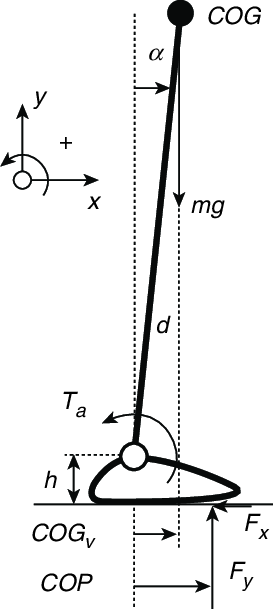
\includegraphics[width=0.3\textwidth]{figures/single_inverted_pendulum.png}}
    \caption{\label{fig:inverted_pendulum} Singolo pendolo inverso}
\end{figure}

Secondo la meccanica classica di Newton-Eulero è possibile descrivere la dinamica del sistema utilizzando la seguente equazione:
\begin{equation}
    {d^2COG\ped{v} \over dt^2} \approx {mgh \over I}(COG\ped{v}-COP)
    \label{eq:approx_cogv}
\end{equation}
dove: $COG\ped{v}$ è la proiezione del centro di gravità sul piano parallelo al terreno, $COP$ è la proiezione del centro di pressione sul piano parallelo al terreno, $h$ è la distanza tra la caviglia e il baricentro e $I$ è il momento d'inerzia del corpo attorno alla caviglia

Possiamo riscrivere l'equazione \ref{eq:approx_cogv} anche come:
\begin{equation}
    {COG\ped{v}(\omega) \over COP(\omega)} = {\omega\ped{0}^2 \over \omega^2+\omega\ped{0}^2}
    \label{eq:cogv_polar}
\end{equation}
dove $\omega$ rappresenta la frequenza angolare e $w\ped{0} = \sqrt{mgh \over I}$ è la frequenza naturale del pendolo inverso. Si noti che all'aumentare della frequenza l'output del sistema diminuisce gradualmente seguendo il comportamento di un filtro passa basso; la proiezione del centro di gravità nel dominio della frequenza può essere considerata come una versione filtrata del centro di pressione.

{\itshape Infine è importante ricordare che il processo di modellizzazione del corpo umano come un singolo pendolo inverso è tutt'altro che completo, specialmente per quanto riguarda la coordinazione e i modelli di controllo; fra i tentativi di miglioramento dell'accuratezza dei modelli troviamo il doppio pendolo inverso.}

\section{Dati ottenuti dall'analisi}
Tipicamente dall'esame stabilometrico si producono due tipi di grafico (esempio in Figura \ref{fig:statokinesigramma}):
\begin{itemize}    
    \item lo {\bfseries statokinesigramma}, detto anche sway-path, raffigura lo spostamento del $COP$ nel piano $xy$
    \item lo {\bfseries stabilogramma} mostra la variazione del $COP$ nel tempo
\end{itemize}

Il $COP$ è espresso sotto forma di vettore in due dimensioni: {\bfseries\itshape Antero-Posteriore} ({\itshape AP}) e {\bfseries\itshape Medio-Laterale} ({\itshape ML}).

\begin{figure}[!htb]
    \center{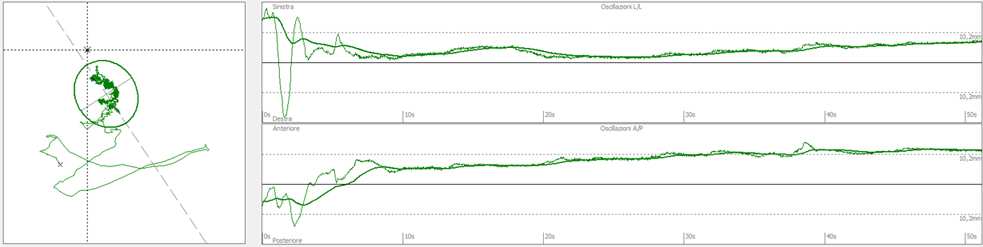
\includegraphics[width=\textwidth]{figures/statokinesigramma.jpg}}
    \caption{\label{fig:statokinesigramma} Esempio di statokinesigramma (sulla sinistra) e di stabilogramma (sulla destra)}
\end{figure}

Dallo statokinesigramma possiamo estrarre diversi parametri utili, questi possono essere classificati in due categorie: {\bfseries parametri globali} e {\bfseries parametri strutturali}; i primi studiano lo sway-pattern nella sua totalità, mentre i secondi si concentrano nel suddividere le traiettorie in pezzetti più piccoli ed estrarre da essi dati utili.

Prima di tutto è importante ricordare che lo scopo di questa tesi è lo sviluppo di un'applicazione per smartphone in grado di determinare la postura e per fare ciò i dati del COP sono ricavati partendo dai valori dell'accelerometro presente nel dispositivo; ci concentreremo solo su alcuni parametri delineando le features da calcolare come:
\begin{enumerate}
    \item Features nel dominio del tempo
    \item Features nel dominio della frequenza
    \item Features strutturali
    \item Features giroscopiche
\end{enumerate}

Le {\itshape features nel dominio del tempo} contengono tutti i parametri ricavati dallo studio del comportamento dello sway-path nel tempo: 
\begin{itemize}
    \item Sway path -> lunghezza della traiettoria del $COP$ nel tempo
    \item Mean distance -> distanza media dal centro del $COP$
    \item Standard deviation of the displacement -> deviazione standard del displacement totale del $COP$
    \item Range -> massima distanza tra due punti del $COP$
\end{itemize}

Le {\itshape features nel dominio della frequenza} si ricavano dalla frequenza dello sway-path, il loro scopo principale è quello di avere una stima dell'energia dello sway-path e di come essa è concentrata nelle varie frequenze:
\begin{itemize}
    \item Frequency at 80\% -> banda di frequenza che contiene l'80\% della frequenza nello spettro AP e ML
    \item Mean frequency -> media della frequenza nello spettro AP e ML
    \item Frequency peak -> i picchi della frequenza nello spettro AP e ML
\end{itemize}

Le {\itshape features strutturali} studiano la sway density curve (SDC) definita come la curva, tempo-indipendente, che per ogni istante temporale conta il numero di campioni consecutivi dello statokinesigramma all'interno di un cerchio di dato raggio. Gli indicatori ricavati sono i seguenti:
\begin{itemize}
    \item np -> numero medio di picchi nella SDC
    \item mean time -> media della distanza temporale fra due picchi della SDC
    \item std time -> deviazione standard di mean time
    \item mean peak -> durata media dei picchi della SDC
    \item sdt peak -> deviazione standard dei mean peak
    \item mean distance -> media della distanza spaziale fra due picchi della SDC
    \item std distance -> deviazione standard di mean distance
\end{itemize}

A differenza delle precedenti le {\itshape features giroscopiche} studiano diversi parametri partendo dai dati del giroscopio
\begin{itemize}
    \item Gyroscope mean -> valore medio del segnale del gyroscope negli assi x,y,z
    \item Gyroscope range -> range del segnale del gyroscope negli assi x,y,z
    \item Gyroscope variance -> varianza del segnale del gyroscope negli assi x,y,z
    \item Gyroscope kurtosis -> indice di curtosi del segnale del gyroscope negli assi x,y,z
    \item Gyroscope skewness -> indice d'asimmetria del segnale del gyroscope negli assi x,y,z
\end{itemize}